\documentclass[aspectratio=169,11pt]{beamer}

% Shared style (ib-tutorials.sty at the repo root).
\makeatletter\def\input@path{{./}{../}}\makeatother
\usepackage{ib-tutorials}

\usepackage[utf8]{inputenc}
\usepackage{amsmath,amssymb}
\usepackage{booktabs}
\usepackage{array}
\newcolumntype{L}[1]{>{\raggedright\arraybackslash}p{#1}}
\usepackage{graphicx}
\graphicspath{{../pictures/3-ibamr-fundamentals/}{pictures/3-ibamr-fundamentals/}}
\usepackage{xcolor}
\usepackage{listings}
\usepackage{tikz}
\usetikzlibrary{arrows.meta,positioning,shapes.geometric,fit,calc}
\usepackage{hyperref}

\newcommand{\sourcecredit}[1]{\vfill\begin{flushright}\tiny\textcolor{DarkGray}{#1}\end{flushright}}

\lstset{
  basicstyle=\ttfamily\scriptsize\color{BlackGray},
  keywordstyle=\color{NavyBlue}\bfseries,
  commentstyle=\color{DarkGray}\itshape,
  stringstyle=\color{OliveGreen},
  showstringspaces=false,
  columns=fullflexible,
  keepspaces=true,
  breaklines=true,
  breakindent=1em,
  frame=single,
  framerule=0.4pt,
  rulecolor=\color{LightGray},
  backgroundcolor=\color{LightGray!30},
  xleftmargin=0.25em,
  xrightmargin=0.25em
}
\lstdefinestyle{shell}{morecomment=[l]{\#}}
\lstdefinestyle{input}{morecomment=[l]{//}}
\lstdefinestyle{matlab}{morecomment=[l]{\%}}
\lstdefinestyle{python}{morecomment=[l]{\#}}
\lstdefinestyle{data}{}
\lstdefinestyle{tiny}{basicstyle=\ttfamily\tiny\color{BlackGray}}
\lstdefinestyle{inputtiny}{morecomment=[l]{//},basicstyle=\ttfamily\tiny\color{BlackGray}}
\lstdefinestyle{matlabtiny}{morecomment=[l]{\%},basicstyle=\ttfamily\tiny\color{BlackGray}}
\lstdefinestyle{pythontiny}{morecomment=[l]{\#},basicstyle=\ttfamily\tiny\color{BlackGray}}
\lstdefinestyle{cpp}{language=C++,morecomment=[l]{//}}
\lstdefinestyle{cpptiny}{language=C++,morecomment=[l]{//},basicstyle=\ttfamily\tiny\color{BlackGray}}
\lstdefinestyle{cmake}{morecomment=[l]{\#}}

\title[Resting curvature and beams]{Resting curvature and beams}
\subtitle{Bending energy, IBAMR's beams and their preferred curvature, a curling beam, and a 2D jellyfish that swims by changing its curvature}
\author[Miller]{Laura A. Miller}
\institute[UArizona]{Department of Mathematics, University of Arizona}
\date{Using IB Software \textbullet\ Part III \textbullet\ Chapter 10}

\begin{document}

% 1
\begin{frame}[plain]
\maketutorialtitlepanel{%
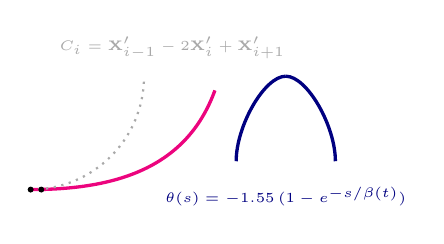
\begin{tikzpicture}[scale=0.9]
  \draw[RubineRed,very thick] (0,0) .. controls (1.2,0) and (2.2,0.3) .. (2.6,1.4);
  \draw[DarkGray,thick,dotted] (0,0) arc (-90:0:1.6);
  \fill[black] (0,0) circle (1.2pt); \fill[black] (0.15,0) circle (1.2pt);
  \node[font=\tiny,text=DarkGray] at (2.0,2.0) {$C_i = \mathbf{X}'_{i-1} - 2\mathbf{X}'_i + \mathbf{X}'_{i+1}$};
  \draw[NavyBlue,very thick] (3.6,1.6) .. controls (3.9,1.6) and (4.3,0.9) .. (4.3,0.4);
  \draw[NavyBlue,very thick] (3.6,1.6) .. controls (3.3,1.6) and (2.9,0.9) .. (2.9,0.4);
  \node[font=\tiny,text=NavyBlue] at (3.6,-0.1) {$\theta(s) = -1.55\,(1 - e^{-s/\beta(t)})$};
\end{tikzpicture}}
\end{frame}

% 2
\begin{frame}{Learning goals}
\label{fr:goals}
\footnotesize By the end of this chapter you should be able to:
\begin{enumerate}
  \item say where the IB method's elastic forces come from (an energy of the point positions, differentiated), and write the stretching and bending energies of a chain of points;
  \item read IBAMR's beam force, $\mathbf{F} = k_b\,(\mathbf{X}_{i-1} - 2\mathbf{X}_i + \mathbf{X}_{i+1} - \mathbf{C}_i)$ on the middle point and its share on the neighbours, and say what the preferred curvature $\mathbf{C}_i = (C_1, C_2)$ is, in what units, and why it depends on the orientation of the body;
  \item give a beam a resting curvature in the \code{.beam} file, and change it in time from an update function with \code{IBBeamForceSpec}, as chapter 9a changed target points and springs;
  \item run the curling beam (IB/09), which curls from straight into a quarter circle, and the jellyfish bell (IB/10), which swims by contracting and expanding its preferred shape;
  \item recognize the two things that go wrong most: a beam too soft to impose its curvature on the fluid in the time available, and a time step too long for the stiffness that would.
\end{enumerate}
\begin{punchbox}
\footnotesize Chapter 9a prescribed positions (target points) and chapter 9b forces (springs). This chapter prescribes \emph{shape}: the third way to make a structure move, and the one that lets a body swim without being told where to go.
\end{punchbox}
\end{frame}

% 3
\begin{frame}{How this chapter was checked}
\label{fr:checked}
\begin{itemize}\footnotesize
  \item The beam force, the meaning of the curvature columns of the \code{.beam} file and the \code{IBBeamForceSpec} accessors are quoted from the IBAMR 0.19.0 sources (\code{IBStandardForceGen.cpp}, \code{IBStandardInitializer.cpp}, \code{IBBeamForceSpec.h}); the three generations of the curvature line in the 2013, 2018 and current code are shown side by side.
  \item The derivations of the 2013 lecture \emph{Bending in IBAMR} (nine slides that were pictures of equations in the course files) are retyped here in full, with the worksheet \code{Discrete\_curvature.xlsx} that went with them.
  \item The two examples are new code built from the course's descriptions, since the course's \code{Example\_2Dbeams\_curvature.zip} and \code{Example\_jellyfish\_curvature.zip} are no longer in the folders: IB/09 (curling beam) from the 2013 \code{update\_beams.C} fragments on the leaf of IB/03, and IB/10 (jellyfish bell) from the 2013 bell description and its \code{update\_beams.C} fragments. Both build with 0 warnings and run to the end; the figures are from those runs, and the parameters that did \emph{not} work are reported.
  \item The Python generators write files identical to the MATLAB ones (Octave 8.4 against Python 3.12).
\end{itemize}
\begin{punchbox}
\footnotesize Slide numbers refer to this deck; chapter numbers (4e, 6, 8a, 8b, 9a, 9b, 11, 16, 36) to the other chapters of this series.
\end{punchbox}
\end{frame}

% 4
\begin{frame}{Where to look things up}
\label{fr:lookup}
\small
\begin{itemize}
  \item \al{The beam force}: \code{src/IB/IBStandardForceGen.cpp}, the function that computes the beam forces (search for \code{curvatures}); the force is five lines (slide \ref{fr:verified}).
  \item \al{The file format}: \code{src/IB/IBStandardInitializer.cpp}, \code{readBeamFiles}; chapter 6's table; the input keys \code{uniform\_beam\_bend\_rigidity} and \code{uniform\_beam\_curvature}.
  \item \al{The beam data in the program}: \code{include/ibamr/IBBeamForceSpec.h}: \code{getMeshDependentCurvatures()}, \code{getBendingRigidities()}, \code{getNeighborNodeIndices()}.
  \item \al{The examples of this series}: IB/09 (curling beam: \code{update\_beams.cpp}, the quarter circle), IB/10 (jellyfish bell: \code{bell\_geometry.h}, \code{update\_beams.cpp}, the pulse), both with READMEs that record what was measured; IB/03 (the leaf these build on) and chapter 8a's stiffness sweep of it.
  \item \al{The physics}: Peskin, \emph{The immersed boundary method}, Acta Numerica 2002 (the energy formulation); Herschlag and Miller, \emph{Reynolds number limits for jet propulsion: a numerical study of simplified jellyfish}, J.\ Theor.\ Biol.\ 2011 (the bell of IB/10).
  \item The IBAMR FAQ, \url{https://github.com/IBAMR/IBAMR/wiki/FAQ}, and the class documentation, \url{https://ibamr.github.io/docs}.
\end{itemize}
\end{frame}

% 5
\begin{frame}{Euler--Bernoulli beam theory}
\label{fr:eb}
\small From the February 2013 lecture \emph{Bending in IBAMR}: ``Comes up often in engineering applications. Assume small deformations and infinitely thin.'' The \al{static beam equation}:
\[
  \frac{d^2}{dx^2}\!\left(EI(x)\,\frac{d^2 y(x)}{dx^2}\right) = f(x), \qquad\text{and if $EI$ is not a function of $x$:}\qquad EI\,\frac{d^4 y(x)}{dx^4} = f(x).
\]
\begin{itemize}
  \item ``$y(x)$ gives deflection of beam in $y$-direction; $x$ gives the length along the beam;
  \item $EI$ is the flexural stiffness (elastic modulus $\times$ second moment of area);
  \item $f(x)$ = force per unit length, may vary along the beam.''
\end{itemize}
\vspace{1mm}
\begin{punchbox}
\small Read it the other way round: a beam bent into the shape $y(x)$ exerts the force per unit length $f = EI\,y''''$ on whatever bends it. In the IB method that ``whatever'' is the fluid, and the beam's own preferred shape enters by replacing $y$ with the deviation from it. The rest of this chapter is the discrete version of this sentence.
\end{punchbox}
\end{frame}

% 6
\begin{frame}{Energy formulations}
\label{fr:energy}
\small ``To specify the elastic properties of the immersed boundaries, an energy function of the immersed boundary point coordinates is created, and the elastic forces that act on the immersed boundary points are calculated from the derivatives of the energy function.
\vspace{1mm}

Typically, the energy function has three contributions: energy from stretching springs, energy from bending the entity, and energy from moving the entity away from a specified location.
\vspace{1mm}

We could go back and derive the energy formulations for linear springs as well.'' (2013)
\vspace{2mm}

\footnotesize The three contributions are chapter 6's three files: \code{.spring} (stretching), \code{.beam} (bending) and \code{.target} (a specified location). Every force IBAMR's standard force generator computes is minus the gradient of one of these energies with respect to the position of a point; the next slides write the three energies and take the derivatives.
\end{frame}

% 7
\begin{frame}{Hooke's law springs}
\label{fr:hooke}
\small
\begin{itemize}
  \item ``Assume that the elastic links which generate the stretching energy act as Hooke's Law Springs.
  \item This means that if elastic link $l$ connects immersed boundary points with indices $p_1(l)$ and $p_2(l)$ and with coordinates $\mathbf{X}_{p_1(l)}$ and $\mathbf{X}_{p_2(l)}$, respectively, then the appropriate energy function for this link is:
\[
  E_S\!\left(\mathbf{X}_{p_1(l)}, \mathbf{X}_{p_2(l)}\right) = \tfrac12\,k_s\left[\left\|\mathbf{X}_{p_1(l)} - \mathbf{X}_{p_2(l)}\right\| - R_l\right]^2
\]
  \item where $R_l$ is the link's resting length, $k_s$ is its stiffness coefficient, and $\|\mathbf{X}\|$ denotes the length of the vector $\mathbf{X}$.'' (2013)
\end{itemize}
\vspace{1mm}
\footnotesize Differentiating with respect to $\mathbf{X}_{p_1}$ gives $-\mathbf{F}_{p_1} = k_s\,(\|\mathbf{X}_{p_1} - \mathbf{X}_{p_2}\| - R_l)\,(\mathbf{X}_{p_1} - \mathbf{X}_{p_2})/\|\mathbf{X}_{p_1} - \mathbf{X}_{p_2}\|$: the tension $T = k_s(R - R_l)$ of chapter 9b's default spring function, along the unit vector between the points. The energy is a function of the distance only, so it does not care how the link is oriented.
\end{frame}

% 8
\begin{frame}{Bending energy with torsional springs}
\label{fr:torsion}
\small
\begin{itemize}
  \item ``The bending energy involves a pair of links emanating from the same immersed boundary point.
  \item It is designed to penalize deviations in the angle between these links from a prescribed angle.
  \item Suppose that immersed boundary points $\mathbf{X}_p$ and $\mathbf{X}_q$ are joined by an elastic link, as are points $\mathbf{X}_q$ and $\mathbf{X}_r$.
  \item The bending energy of this triple of points is:
\[
  E_B(\mathbf{X}_p, \mathbf{X}_q, \mathbf{X}_r) = \tfrac12\,k_b\left[\mathbf{z}\cdot(\mathbf{X}_r - \mathbf{X}_q)\times(\mathbf{X}_q - \mathbf{X}_p) - C\right]^2
\]
  \item where $k_b$ is the bending stiffness, $C$ is a specified `curvature', and $\mathbf{z} = (0,0,1)$.'' (2013)
\end{itemize}
\vspace{1mm}
\small In two dimensions the triple product is a scalar and the energy is
\[
  E_B(\mathbf{X}_p, \mathbf{X}_q, \mathbf{X}_r) = \tfrac12\,k_b\left[(x_r - x_q)(y_q - y_p) - (y_r - y_q)(x_q - x_p) - C\right]^2 .
\]
\end{frame}

% 9
\begin{frame}{2D bending energy: what $C$ means}
\label{fr:angle}
\begin{columns}[T,onlytextwidth]
\begin{column}{0.62\textwidth}
\small ``In 2D, the energy formulation for the torsional springs is'' the one above. ``$C$ is a `curvature' that can be determined by the desired angle made by this triplet. This formulation has the advantage that it is easy to conceptualize and does not depend upon the orientation relative to the coordinate system.'' (2013)
\vspace{1mm}

\small \al{Minimizing bending energy.} ``Recall the geometric definition of the cross product $\mathbf{a}\times\mathbf{b}$'': its magnitude is $\|\mathbf{a}\|\|\mathbf{b}\|\sin\theta$. ``This function achieves its minimum value when the exterior angle between the links satisfies
\[
  \theta = \sin^{-1}\!\left(\frac{C}{\|\mathbf{X}_r - \mathbf{X}_q\|\,\|\mathbf{X}_q - \mathbf{X}_p\|}\right).\text{''}
\]
\end{column}
\begin{column}{0.36\textwidth}
\centering
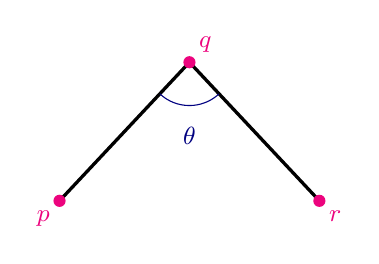
\begin{tikzpicture}[scale=1.1]
  \draw[very thick] (0,0) -- (1.5,1.6) -- (3.0,0);
  \fill[RubineRed] (0,0) circle (2pt) node[below left,font=\small] {$p$};
  \fill[RubineRed] (1.5,1.6) circle (2pt) node[above right,font=\small] {$q$};
  \fill[RubineRed] (3.0,0) circle (2pt) node[below right,font=\small] {$r$};
  \draw[NavyBlue] (1.5,1.6) ++(-133:0.5) arc (-133:-47:0.5);
  \node[font=\small,text=NavyBlue] at (1.5,0.75) {$\theta$};
\end{tikzpicture}

\vspace{2mm}
\footnotesize The 2013 figure: the exterior angle $\theta$ at $q$ between the links $pq$ and $qr$. $C = 0$ asks for a straight line; $C > 0$ bends one way, $C < 0$ the other, and the sign does not change when the whole triple is rotated. This is the beam of IB2d (chapter 4e), which has both this form and IBAMR's.
\end{column}
\end{columns}
\end{frame}

% 9b
\begin{frame}{Minimizing bending energy: setting $C$ from the angle}
\label{fr:angle2}
\small ``If the angle between the pair of links differs from $\theta_{\mathrm{desired}}$, the force associated with the energy drives the angle toward $\theta_{\mathrm{desired}}$. If the resting lengths for the links in the triple are $R_{pq}$ and $R_{qr}$, then in order to set the desired angle to $\theta_{\mathrm{desired}}$, $C$ should be set to
\[
  C = R_{pq}\,R_{qr}\,\sin(\theta_{\mathrm{desired}}).
\]
Typically, the three points in the bending energy formula are consecutive points of a given immersed boundary entity. The bending stiffness $k_b$ and desired curvature $C$ can vary from triplet to triplet.'' (2013)
\vspace{2mm}

\footnotesize For a smooth curve of curvature $\kappa$ sampled $\Delta s$ apart, the exterior angle between consecutive links is $\theta \approx \kappa\,\Delta s$, so $C \approx \Delta s^2\,\kappa$: the same magnitude as IBAMR's $\|\mathbf{C}\|$ of slide \ref{fr:worksheet}, but a scalar with a sign instead of a vector with a direction. That is the whole difference between the two formulations, and the reason one is orientation-free and the other is not.
\end{frame}

% 10
\begin{frame}{Calculating the total energy and the force}
\label{fr:total}
\small ``The elastic energy is the sum of the stretching and bending energies for each immersed boundary point. If there are $N$ immersed boundary points arranged in the order $\mathbf{X}_1, \mathbf{X}_2, \mathbf{X}_3, \ldots, \mathbf{X}_N$; that each pair of consecutive points is joined by an elastic link; that each consecutive triple has an associated bending energy. Then the elastic energy is:
\[
  E(\mathbf{X}_1, \mathbf{X}_2, \ldots, \mathbf{X}_N) = \sum_{q=1}^{N-\delta} E_S(\mathbf{X}_q, \mathbf{X}_{q+1}) + \sum_{q=1+\delta}^{N-\delta} E_B(\mathbf{X}_{q-1}, \mathbf{X}_q, \mathbf{X}_{q+1}),
\]
$\delta = 0$ if there is a spring connecting $\mathbf{X}_1$ with $\mathbf{X}_N$, and $\delta = 1$ otherwise.'' (A closed loop, like IB/01's band, has a spring and a beam across the join; an open fibre, like IB/03's leaf, has one spring and one beam fewer.)
\vspace{1mm}

``The elastic force at point $p$, $\mathbf{F}_p$, is then calculated from the derivatives of the elastic energy, $E(\mathbf{X}, t)$, with respect to the coordinates in $\mathbf{X}_p$:
\[
  \mathbf{F}_p(\mathbf{X}, t) = -\frac{\partial E(\mathbf{X}, t)}{\partial \mathbf{X}_p}.
\]
The minus sign is chosen to drive the system towards a minimum of the energy.'' (2013)
\end{frame}

% 11
\begin{frame}{Energy formulation for continuous beams}
\label{fr:continuous}
\small ``With zero preferred curvature, the bending energy is given by:
\[
  E_b = \tfrac12\,k_b \int \left|\frac{\partial^2 \mathbf{X}(s,t)}{\partial s^2}\right|^2 ds .
\]
One can then discretize the bending energy with zero preferred curvature as:
\[
  E_b = \tfrac12\,k_b \sum_i \left|D_s D_s \mathbf{X}\right|^2 \Delta s
      = \tfrac12\,k_b \sum_{i=2}^{N-1} \left[\frac{\left|\mathbf{X}_{i+1} - 2\mathbf{X}_i + \mathbf{X}_{i-1}\right|^2}{(\Delta s)^4}\right] \Delta s .\text{''}
\]
\vspace{1mm}
\footnotesize $D_s$ is the difference along the fibre; applied twice it gives the second difference over $(\Delta s)^2$, whose square over $(\Delta s)^4$ is the integrand. The sum runs over the interior points, each of which is the middle of one beam; the $\Delta s$ at the end is the integral's $ds$. IBAMR folds the $(\Delta s)^4$ and the $\Delta s$ into the file's stiffness, $k_b/\Delta s^3$ (slide \ref{fr:verified}).
\end{frame}

% 12
\begin{frame}{Calculating the forces of the discrete beam}
\label{fr:discreteforce}
\small ``The elastic force at point $p$, $\mathbf{F}_p$, is then calculated from the derivatives of the elastic energy with respect to the coordinates in $\mathbf{X}_p$:
\[
  (\mathbf{F}_b)_p = \frac{k_b}{(\Delta s)^4} \sum_{i=2}^{N-1} \left(\mathbf{X}_{i+1} - 2\mathbf{X}_i + \mathbf{X}_{i-1}\right)\left(2\delta_{i,p} - \delta_{i+1,p} - \delta_{i-1,p}\right),
\]
where $\delta$ is the Kronecker symbol whose definition is
\[
  \delta_{i,p} = \begin{cases} 1, & \text{if } i = p\\ 0, & \text{if } i \neq p. \end{cases}\text{'' (2013)}
\]
\vspace{1mm}
\footnotesize Read the sum for one point $p$: the triple centred on $p$ ($i = p$) contributes $+2$ times its second difference, and the two triples that have $p$ as a neighbour ($i = p \pm 1$) contribute $-1$ times theirs. That is exactly the ``$+2$ on the master, $-1$ on each neighbour'' of IBAMR's code (slide \ref{fr:verified}), with the $(\Delta s)^4$ and the $\Delta s$ of the energy folded into the file's stiffness. (The sign: this $\mathbf{F}_b$ is $-\partial E_b/\partial\mathbf{X}_p$ up to the convention for the second difference; IBAMR's five lines settle it.)
\end{frame}

% 13
\begin{frame}{IBAMR beams with nonzero curvature}
\label{fr:nonzero}
\small ``In IBAMR, the equation describing the force along the boundary due to bending is given by
\[
  \mathbf{F}(s,t) = -k_b\,\frac{\partial^4}{\partial s^4}\big(\mathbf{X}(s,t) - \mathbf{X}_b(s,t)\big) = -k_b\left(\frac{\partial^4 \mathbf{X}(s,t)}{\partial s^4} - \frac{\partial^4 \mathbf{X}_b(s,t)}{\partial s^4}\right)
\]
where $s$ represents the position along the fiber and $\mathbf{X}_b(s,t)$ specifies the curvature of the fiber.
\begin{itemize}
  \item There is an issue that $\mathbf{X}_b$ depends on the orientation relative to the coordinate system.
  \item For rotating boundaries, $\mathbf{X}_b$ would need to be updated over time.
  \item If the curvature is zero, there is no issue.'' (2013)
\end{itemize}
\vspace{1mm}
\begin{punchbox}
\small $\mathbf{X}_b$ is a \emph{preferred shape}, given as positions; only its fourth derivative (its second difference, once discretized) matters, so where the shape sits does not matter but how it is turned does. A fibre that rotates with the flow (a free-swimming body that yaws) keeps a preferred shape fixed in the laboratory frame unless the program rotates $\mathbf{X}_b$ with it: slide \ref{fr:orientation}. The angle formulation of slide \ref{fr:angle} has no such issue, and IBAMR does not offer it.
\end{punchbox}
\end{frame}

% 14
\begin{frame}{IBAMR curvatures, $C_1$ and $C_2$}
\label{fr:c1c2}
\small ``The bending energy formulation is:
\[
  E_B(\mathbf{X}_p, \mathbf{X}_q, \mathbf{X}_r) = \tfrac12\,k_b\left(\frac{\left|(\mathbf{x}_{i-1} - 2\mathbf{x}_i + \mathbf{x}_{i+1}) - \mathbf{C}\right|^2}{(\Delta s)^4}\right)\Delta s
\]
where $\mathbf{C} = (C_1, C_2)$ is given by
\[
  C_1 = x'_{i-1} - 2x'_i + x'_{i+1}, \qquad C_2 = y'_{i-1} - 2y'_i + y'_{i+1},
\]
and $\mathbf{x}' = (x', y')$ are the preferred configurations of the boundary.'' (2013)
\vspace{1mm}

\footnotesize So the preferred curvature of beam $i$ is the \al{second difference of the preferred positions} of its three points. It is a vector with the units of length (metres in the examples), not a curvature in $1/\mathrm{m}$: for points $\Delta s$ apart on a curve of curvature $\kappa$ its magnitude is $\kappa\,\Delta s^2$ (next slide), and its direction is the normal of the preferred shape, in laboratory coordinates. The generator computes it from the shape it wants (IB/10's bell) and an update function recomputes it when the shape changes (IB/09, IB/10).
\end{frame}

% 15
\begin{frame}[fragile]{What IBAMR computes, from the source}
\label{fr:verified}
\begin{columns}[T,onlytextwidth]
\begin{column}{0.55\textwidth}
\begin{lstlisting}[style=cpptiny]
// src/IB/IBStandardForceGen.cpp (0.19.0), the beam loop (2D lines)
K = *rigidities[k];             // the beam's stiffness, from the .beam file
D2X0 = curvatures[k]->data();   // its preferred curvature (C1, C2)
F[0] = K * (X_node[next_idx + 0] + X_node[prev_idx + 0]
            - 2.0 * X_node[mastr_idx + 0] - D2X0[0]);
F[1] = K * (X_node[next_idx + 1] + X_node[prev_idx + 1]
            - 2.0 * X_node[mastr_idx + 1] - D2X0[1]);
F_node[mastr_idx + 0] += 2.0 * F[0];
F_node[mastr_idx + 1] += 2.0 * F[1];
F_node[next_idx + 0] -= F[0];
F_node[next_idx + 1] -= F[1];
F_node[prev_idx + 0] -= F[0];
F_node[prev_idx + 1] -= F[1];
\end{lstlisting}
\footnotesize In words: for beam $k$ with master (middle) point $i$ and neighbours $i \pm 1$,
\[
  \mathbf{F} = K\,(\mathbf{X}_{i+1} + \mathbf{X}_{i-1} - 2\mathbf{X}_i - \mathbf{C}_i),
\]
and the middle point receives $+2\mathbf{F}$, each neighbour $-\mathbf{F}$. The three forces sum to zero (no net force or torque from a beam on itself).
\end{column}
\begin{column}{0.43\textwidth}
\scriptsize What this fixes about units and signs:
\begin{itemize}
  \item $K$ is the number in the \code{.beam} file. Comparing with slide \ref{fr:discreteforce}, $K = k_b/\Delta s^3$: the generators write \code{kappa\_beam*ds/ds\^{}4}, and chapter 6's rule ``beam stiffness divided by $\Delta s^3$'' is this line.
  \item $\mathbf{C}_i$ is compared directly with $\mathbf{X}_{i+1} + \mathbf{X}_{i-1} - 2\mathbf{X}_i$, so it has the units of $\mathbf{X}$ and the same orientation as $\mathbf{X}$. If the beam already has the second difference $\mathbf{C}_i$, the force is zero: a bent beam at rest.
  \item A beam with $\mathbf{C}_i = 0$ is pushed straight; this is what every \code{.beam} file of chapters 6--9 asked for.
  \item The middle point is pushed \emph{toward} the preferred position relative to its neighbours ($+2\mathbf{F}$ points from $\mathbf{X}_i$ toward the midpoint of the neighbours, shifted by $\mathbf{C}_i$).
\end{itemize}
\end{column}
\end{columns}
\end{frame}

% 16
\begin{frame}{The quarter-circle worksheet: $\|\mathbf{C}\| = \Delta s^2\,\kappa$}
\label{fr:worksheet}
\begin{columns}[T,onlytextwidth]
\begin{column}{0.56\textwidth}
\scriptsize The 2013 worksheet \code{Discrete\_curvature.xlsx}: 100 points $\Delta s = 0.001$ apart on a quarter circle of radius $r = 1/(5\pi) = 0.063662$, so that the arc is $0.1$ long; $x = r\cos\theta$, $y = r\sin\theta$. Its first rows (the slide showed twenty; the sheet has a hundred):
\vspace{1mm}

\setlength{\tabcolsep}{1pt}
\tiny
\begin{tabular}{@{}rrrrrr@{}}
\toprule
$\theta$ & $x(n)$ & $y(n)$ & $C_1$ & $C_2$ & $\|\mathbf{C}\|$\\
\midrule
0 & 0.063662 & 0 & & & \\
0.015708 & 0.063654 & 0.001000 & $-1.57057\times10^{-5}$ & $-2.46725\times10^{-7}$ & $1.57\times10^{-5}$\\
0.031416 & 0.063631 & 0.002000 & $-1.56999\times10^{-5}$ & $-4.93389\times10^{-7}$ & $1.57\times10^{-5}$\\
0.047124 & 0.063591 & 0.002999 & $-1.56902\times10^{-5}$ & $-7.39931\times10^{-7}$ & $1.57\times10^{-5}$\\
0.062832 & 0.063536 & 0.003997 & $-1.56766\times10^{-5}$ & $-9.86291\times10^{-7}$ & $1.57\times10^{-5}$\\
$\vdots$ & & & & & \\
0.282743 & 0.061134 & 0.017761 & $-1.50839\times10^{-5}$ & $-4.38229\times10^{-6}$ & $1.57\times10^{-5}$\\
\bottomrule
\end{tabular}

\vspace{1mm}
\scriptsize $C_1 = x(n+1) - 2x(n) + x(n-1)$, $C_2 = y(n+1) - 2y(n) + y(n-1)$.
\end{column}
\begin{column}{0.42\textwidth}
\small ``$\|\mathbf{C}\|$ is constant along the boundary. $\|\mathbf{C}\|$ can also be related to the curvature, $C$, of the circle: $\|\mathbf{C}\| = C\,\Delta s^2$.'' (2013)
\vspace{1mm}

\footnotesize With $C = 1/r = 15.7$ and $\Delta s^2 = 10^{-6}$: $\|\mathbf{C}\| = 1.57\times10^{-5}$, the last column. The direction of $(C_1, C_2)$ turns with $\theta$ (it points to the centre of the circle), which is the orientation dependence of slide \ref{fr:nonzero} in numbers: rotate the quarter circle by $90^\circ$ and $(C_1, C_2)$ becomes $(-C_2, C_1)$.
\vspace{1mm}

\footnotesize The same worksheet gives the generator's recipe for any preferred shape: place the points on it $\Delta s$ apart, take second differences, write them as columns 5 and 6 of the \code{.beam} file (next slide). IB/10's generator does this for the bell.
\end{column}
\end{columns}
\end{frame}

% 17
\begin{frame}[fragile]{The \code{.beam} file with a resting curvature}
\label{fr:beamfile}
\begin{columns}[T,onlytextwidth]
\begin{column}{0.5\textwidth}
\begin{lstlisting}[style=data]
255
0 1 2 2.0971520000000000e+06 6.3e-06 -1.5e-06
1 2 3 2.0971520000000000e+06 6.3e-06 -1.5e-06
...
\end{lstlisting}
\footnotesize IB/10's \code{bell\_256.beam} (values shortened): \code{i-1 i i+1 stiffness C1 C2}. Without the last two columns (IB/01--IB/09) the preferred curvature is zero.
\vspace{1mm}

\footnotesize From \code{IBStandardInitializer.cpp} (0.19.0):
\begin{itemize}
  \item the stiffness must not be negative (``beam constant is negative'');
  \item then \code{NDIM} more numbers are read if present: in 2D two, in 3D three. One number alone is an error, ``incomplete beam curvature specification'': give all or none;
  \item \code{uniform\_beam\_bend\_rigidity} and \code{uniform\_beam\_curvature} in the structure's input block override every line's stiffness or curvature, like the other \code{uniform\_*} keys of chapter 6.
\end{itemize}
\end{column}
\begin{column}{0.48\textwidth}
\begin{lstlisting}[style=pythontiny]
# generate_mesh2d.py (IB/10): the preferred curvature is the second
# difference of the resting shape, so the bell is at rest at t = 0
with open(f"{mesh_name}{N}.beam", "w", newline="\n") as f:
    f.write("%d\n" % (npts - 2))
    for i in range(1, npts - 1):
        c1 = X[i - 1] - 2 * X[i] + X[i + 1]
        c2 = Y[i - 1] - 2 * Y[i] + Y[i + 1]
        f.write("%d %d %d %1.16e %1.16e %1.16e\n"
                % (i - 1, i, i + 1, kappa_beam * ds / (ds ** 4), c1, c2))
\end{lstlisting}
\footnotesize Two uses of the columns:
\begin{itemize}
  \item a body that is \al{bent at rest}: write its own second differences, as here, and it holds its shape against the flow instead of straightening (a curved fin, a coiled tentacle, the bell);
  \item a body that \al{starts straight but wants to be bent}: write the curvature of the target shape and it curls up at the start (slide \ref{fr:curl2} shows why that is not instant).
\end{itemize}
\end{column}
\end{columns}
\end{frame}

% 18
\begin{frame}[fragile]{Reading and changing the curvature in the program}
\label{fr:api}
\begin{columns}[T,onlytextwidth]
\begin{column}{0.56\textwidth}
\begin{lstlisting}[style=cpptiny]
// include/ibamr/IBBeamForceSpec.h (0.19.0): the beam data stored with a master node
unsigned int getNumberOfBeams() const;
std::vector<NeighborIdxs>& getNeighborNodeIndices();      // (prev, next) of each beam
std::vector<double>& getBendingRigidities();              // the stiffness of each beam
std::vector<IBTK::Vector>& getMeshDependentCurvatures();  // (C1, C2) of each beam, a reference
\end{lstlisting}
\begin{lstlisting}[style=cpptiny]
// update_beams.cpp (IB/09 and IB/10): the pattern of chapter 9a
IBBeamForceSpec* const beam_spec = node->getNodeDataItem<IBBeamForceSpec>();
if (beam_spec == nullptr) continue;          // not the middle point of any beam
const int lag_idx = node->getLagrangianIndex();
...
for (IBTK::Vector& curv : beam_spec->getMeshDependentCurvatures())
{
    curv[0] = ...;   // C1
    curv[1] = ...;   // C2
}
\end{lstlisting}
\end{column}
\begin{column}{0.42\textwidth}
\footnotesize The pattern is chapter 9a's: loop over the local and ghost nodes, ask each for its beam data, skip the nodes that have none, find the point's number along the structure, and write the new values \emph{through the reference}. The force generator reads them at the next force evaluation.
\vspace{1mm}

\footnotesize ``\code{[0]} indicates the first beam, \code{[1]} would be the second. Typically you only have one beam per node.'' (2013) A node has more than one beam only if the generator wrote it as the middle point of several triples (a branching structure); the range-based loop handles any number.
\vspace{1mm}

\footnotesize ``Uncomment below to get bending stiffnesses: \code{std::vector<double>\& kbend = beam\_spec->getBendingRigidities();}'' (2013): the stiffness can change in time the same way (a muscle that stiffens), as chapter 9b's stiffness wave did for springs.
\end{column}
\end{columns}
\end{frame}

% 18b
\begin{frame}[fragile]{The curvature line through three generations of IBAMR}
\label{fr:api2}
\small The course taught the same line three times as IBAMR changed; the 2018 slide kept all three, with ``the newest way uncommented'':
\begin{lstlisting}[style=cpptiny]
//There are three ways to get beam curvatures depending on the IBAMR version.
//The newest way is uncommented.
      //TinyVector<double, 2>& curv = beam_spec->getMeshDependentCurvatures()[0];   // 2013
      //IBTK::Vector<double, 2> curv = beam_spec->getMeshDependentCurvatures()[0];  // intermediate
      Point& curv = beam_spec->getMeshDependentCurvatures()[0];                     // 2018
\end{lstlisting}
\begin{itemize}\footnotesize
  \item The middle version has no \code{\&}: it makes a \al{copy}, and writing to it changes nothing, chapter 9a's copy bug again. Take a reference, or loop over the vector by reference as IB/09 and IB/10 do (\code{for (IBTK::Vector\& curv : ...)}).
  \item \code{Point} and \code{IBTK::Vector} are the same Eigen type today, and \code{IBTK::Vector} is the name in the header; \code{TinyVector} (the 2013 Blitz++ type) is gone. In a \code{.cpp} that includes \code{app\_namespaces.h}, write \code{IBTK::Vector} in full: a bare \code{Vector} is ambiguous between IBTK's and SAMRAI's.
  \item \code{[0]} hard-codes ``the first beam''; the loop form needs no index and no \code{NDIM} assumptions (the 2013 code wrote \code{2} where current code writes \code{NDIM}).
\end{itemize}
\end{frame}

% 19
\begin{frame}[fragile]{The 2013 example: a fiber that curls into a quarter circle}
\label{fr:ex2013}
\begin{columns}[T,onlytextwidth]
\begin{column}{0.48\textwidth}
\footnotesize ``Simple example to change curvature. \code{Example\_2Dbeams\_curvature} is available in the examples folder. The curvature of a 2D fiber is increased at each time step. At $t = 1$ it should form a quarter circle. New files are \code{update\_beams.C} and \code{update\_beams.h}. You also need to add these files to \code{main.C} and \code{input2d}. This is similar to \code{update\_target\_point\_positions}.'' (2013, 2018)
\vspace{1mm}

\footnotesize ``Bending IBAMR beam: simulation with constant $C_1$ and $C_2$. Initialized as a straight horizontal beam.'' (the 2013 picture)
\vspace{1mm}

\footnotesize The 2013 slide also carried a login for a UNC machine and the note that the example ``requires the forcing version of IBAMR''; both are history. The zip is no longer in the course folders, so IB/09 rebuilds it from these fragments.
\end{column}
\begin{column}{0.5\textwidth}
\begin{lstlisting}[style=cpptiny]
// update_beams.C (2013), "updating the curvatures"
// I've set up the code below to set the curvatures of the beam to the
// curvature of a circle whose radius decreases over time.
my_phi0=(lag_idx-1)*(pi/2)/npts;
my_phi1=(lag_idx)*(pi/2)/npts;
my_phi2=(lag_idx+1)*(pi/2)/npts;
// curv[0] would be C1 and curv[1] would be C2
// At t=1, the beam would form a quarter circle.
curv[0]=(current_time/(10*pi/2))*(cos(my_phi0)-2*cos(my_phi1)+cos(my_phi2));
curv[1]=(current_time/(10*pi/2))*(sin(my_phi0)-2*sin(my_phi1)+sin(my_phi2));
\end{lstlisting}
\footnotesize Read it: the three angles are those of points $i-1$, $i$, $i+1$ on a quarter circle of \code{npts} points; the brackets are second differences of $\cos$ and $\sin$, i.e.\ of a unit circle; the prefactor $t/(10\cdot\pi/2) = t/(5\pi)$ is the radius, $1/(5\pi) = 0.0637$ m at $t = 1$: the worksheet's circle. (The comment says ``decreases''; the radius of the \emph{preferred} circle increases from 0 and the curvature the beam feels increases with it, slide \ref{fr:curl1}.) \code{lag\_idx} is the global index, so this works for structure 0 only.
\end{column}
\end{columns}
\end{frame}

% 20
\begin{frame}[fragile]{IB/09, the curling beam: what it is}
\label{fr:curl1}
\begin{columns}[T,onlytextwidth]
\begin{column}{0.5\textwidth}
\footnotesize IB/03's leaf (103 points, $0.1$ m, $\Delta s = 0.98$ mm) laid horizontally in a $1$ m box of still fluid ($\rho = 1000$, $\mu = 0.1$, no-slip walls), clamped at its left end by two target points (position and direction), springs $K = 30$, beams $k_b = 0.02$ (four times the leaf's). Before every step \code{update\_beams} sets each beam's curvature to the second difference of
\[
  \mathbf{X}_i = \big(R\sin\varphi_i,\; R\,(1 - \cos\varphi_i)\big), \quad \varphi_i = \frac{i}{n_{\mathrm{pts}} - 1}\,\frac{\pi}{2},
\]
a quarter circle that leaves the clamp along $+x$ and curls upward, with $R(t) = R_{\mathrm{final}}\min(t/T_{\mathrm{curl}}, 1)$ and $R_{\mathrm{final}} = 0.1/(\pi/2) = 0.0637$ m (the update function is on the next slide).
\vspace{1mm}

\footnotesize Run time: 60,000 steps of $5\times10^{-5}$ s (3 s), about 12 minutes on 3 cores. With the leaf's own stiffness ($k_b = 0.005$) and $\Delta t = 10^{-4}$ it runs too, but lags its shape by 44 mm at $t = 1$ s (slide \ref{fr:curl3}).
\end{column}
\begin{column}{0.48\textwidth}
\footnotesize What the ramp means. The second difference of points $\Delta\varphi$ apart on a circle of radius $R$ has magnitude $R\,\Delta\varphi^2$; the beam's points are $\Delta s$ apart, so the curvature they are asked for is $R\,\Delta\varphi^2/\Delta s^2 = R/R_{\mathrm{final}}^2$: it grows linearly from 0 to $1/R_{\mathrm{final}}$, and the preferred shape at time $t$ is an arc of radius $R_{\mathrm{final}}^2/R(t)$ and length $0.1$ (the dotted curves of the next slide).
\vspace{1mm}

\footnotesize Changes from the 2013 fragments: the point number is counted from the structure's first index (\code{getLagrangianStructureIndexRange}), not the global \code{lag\_idx}; the angle step divides by $n_{\mathrm{pts}} - 1$ gaps, not $n_{\mathrm{pts}}$; \code{T\_CURL} is an input key; the arc starts along the clamp's direction (the worksheet's circle started vertically); ghost nodes are visited (chapter 9a).
\end{column}
\end{columns}
\end{frame}

% 20b
\begin{frame}[fragile]{IB/09: the update function}
\label{fr:curlcode}
\begin{lstlisting}[style=cpptiny]
// update_beams.cpp (IB/09)
const std::pair<int, int> beam_idxs = l_data_manager->getLagrangianStructureIndexRange(0, finest_ln);
const int npts = beam_idxs.second - beam_idxs.first;
const double R_final = beam_length / (M_PI / 2.0);                  // 0.0637 m: the quarter circle of the beam's length
const double R = R_final * std::min(current_time / T_curl, 1.0);    // grows over T_curl, then holds
const double dphi = (M_PI / 2.0) / (npts - 1);
...
for (LNode* const node : nodes)
{
    IBBeamForceSpec* const beam_spec = node->getNodeDataItem<IBBeamForceSpec>();
    if (beam_spec == nullptr) continue;                               // not the middle point of any beam
    const int lag_idx = node->getLagrangianIndex();
    if (lag_idx < beam_idxs.first || lag_idx >= beam_idxs.second) continue;
    const int i = lag_idx - beam_idxs.first;                          // the point's number along the beam
    const double phi0 = (i - 1) * dphi, phi1 = i * dphi, phi2 = (i + 1) * dphi;
    for (IBTK::Vector& curv : beam_spec->getMeshDependentCurvatures())
    {
        curv[0] = R * (std::sin(phi0) - 2.0 * std::sin(phi1) + std::sin(phi2));   // C1
        curv[1] = R * (-std::cos(phi0) + 2.0 * std::cos(phi1) - std::cos(phi2));  // C2
    }
}
\end{lstlisting}
\footnotesize \code{main.cpp} calls it before \code{advanceHierarchy} with \code{loop\_time}, \code{dt} and \code{T\_curl} (read from the input as \code{T\_CURL}), exactly where IB/07 called \code{update\_target\_point\_positions}; \code{CMakeLists.txt} lists the second \code{.cpp}.
\end{frame}

% 21
\begin{frame}{IB/09: the beam and the arc it is asked for}
\label{fr:curl2}
\begin{columns}[T,onlytextwidth]
\begin{column}{0.52\textwidth}
\centering
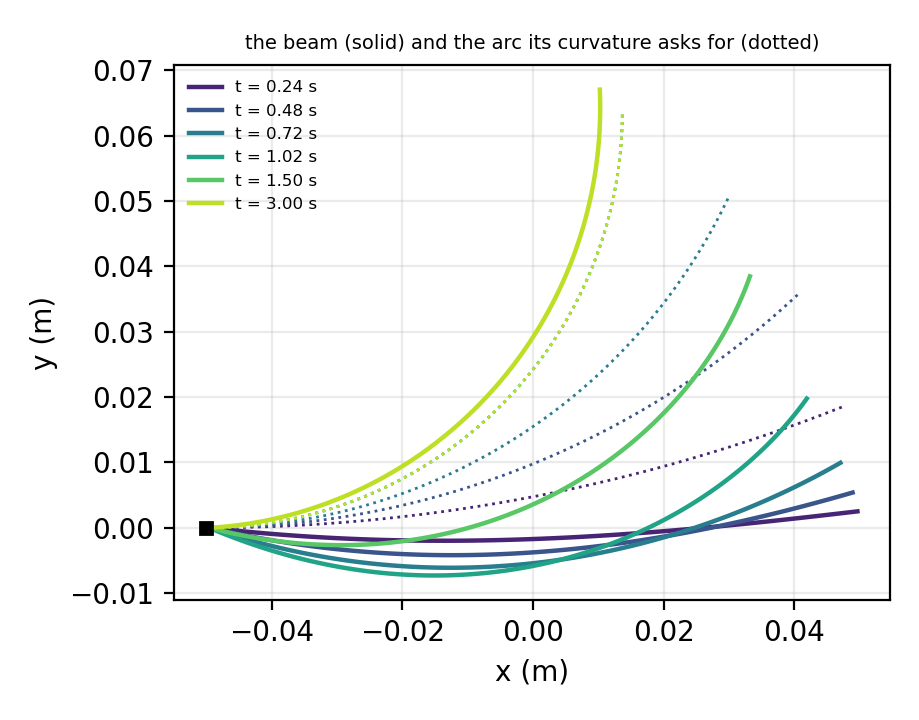
\includegraphics[width=\textwidth]{ch10-curl-shapes}
\end{column}
\begin{column}{0.46\textwidth}
\footnotesize Solid: the beam at six times. Dotted: the arc its curvature asks for at that time (radius $R_{\mathrm{final}}^2/R(t)$, the quarter circle at $t \geq 1$). The square is the clamp. The fluid is IB/03's ($\rho = 1000$, $\mu = 4$).
\begin{itemize}
  \item The beam \al{lags} its preferred shape while the curvature is changing, and catches up once it stops: the fluid has inertia ($\rho = 1000$) and must be pushed out of the way; a stiffer beam pushes harder.
  \item Near the clamp it first dips \emph{below} the line: the curvature pulls the far part up and the reaction, with the clamp holding the base, bends the near part down until the whole beam has turned.
  \item The measured numbers are on the next slide and in the README.
\end{itemize}
\end{column}
\end{columns}
\sourcecredit{IB/09 with IBAMR 0.19.0, $k_b = 0.02$, $\mu = 4$, $\Delta t = 5\times10^{-5}$, 3 s; \code{tools/ch10\_figures.py} reads \code{hier\_data\_IB2d/X.*}.}
\end{frame}

% 22
\begin{frame}{IB/09: how closely the beam follows}
\label{fr:curl3}
\begin{columns}[T,onlytextwidth]
\begin{column}{0.6\textwidth}
\centering
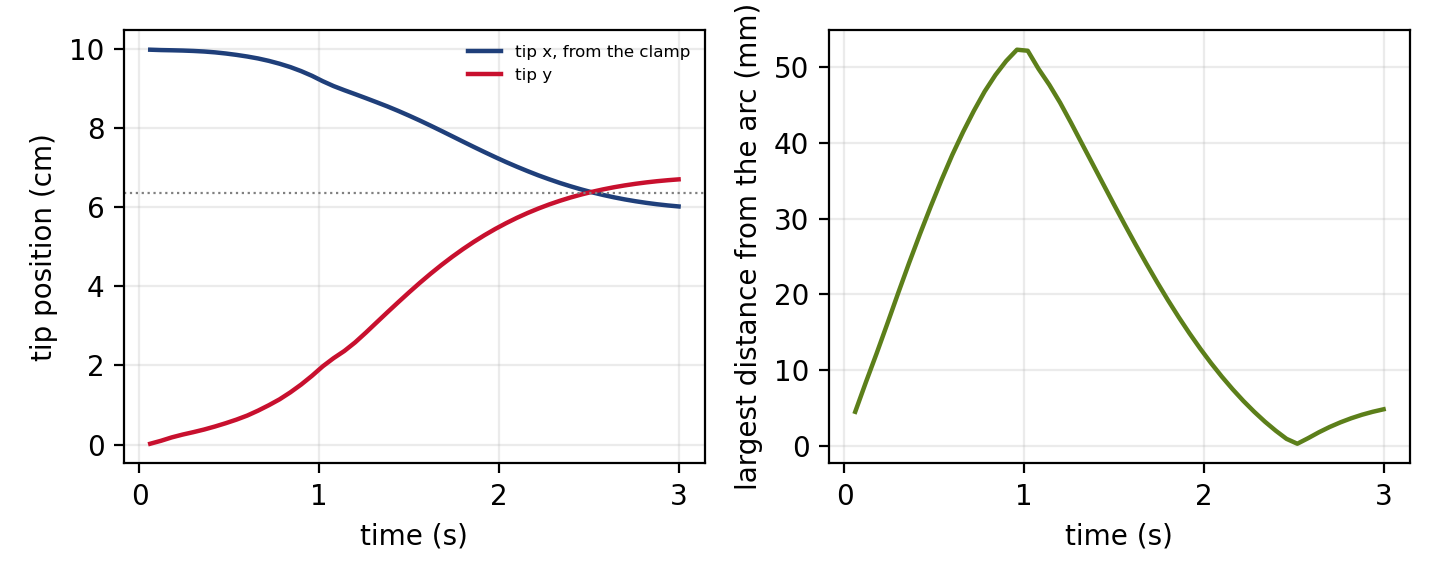
\includegraphics[width=\textwidth]{ch10-curl-tip}
\end{column}
\begin{column}{0.38\textwidth}
\scriptsize Left: the tip's position relative to the clamp; the dotted line is $R_{\mathrm{final}} = 6.37$ cm, where both coordinates end up for a quarter circle. Right: the largest distance between any point of the beam and the arc its curvature asks for.
\vspace{1mm}

\scriptsize Measured ($\mu = 4$, $k_b = 0.02$): the beam is $3.2$ cm from its arc at $0.5$ s, $4.4$ cm at $0.75$ s and $5.2$ cm at $1$ s, when the curvature stops changing; it then closes in ($3.2$ cm at $1.5$ s, $1.3$ cm at $2$ s) and settles within $5$ mm of the quarter circle by $2.5$ s. With $\mu = 1$ the lag at $1$ s is $4.1$ cm and the settling is the same; with $\mu = 0.1$ the beam overshoots and oscillates about the circle with a period of about $1$ s.
\vspace{1mm}

\scriptsize Two ways to make it follow more closely: a stiffer beam (with a shorter time step: $k_b \times 10$ needs $\Delta t = 2.5\times10^{-5}$ in chapter 8a's leaf sweep) or a slower curl (\code{T\_CURL = 2}). The lag is dynamic, not a steady offset: at rest, a beam with no load takes exactly its preferred shape whatever $k_b$ is.
\end{column}
\end{columns}
\sourcecredit{Same run; \code{tools/ch10\_figures.py}.}
\end{frame}

% 23
\begin{frame}{A specific example: jellyfish swimming by prescribing curvature}
\label{fr:jelly1}
\begin{columns}[T,onlytextwidth]
\begin{column}{0.5\textwidth}
\scriptsize From the February 2013 lecture \emph{Specific example of jellyfish swimming by prescribing curvature} and its 2018 edition: ``This example can be downloaded from the Examples folder as \code{Example\_jellyfish\_curvature.zip}.''
\vspace{1mm}

\footnotesize ``\al{Describing the bell position.} The tangent angle $\theta$ is horizontal at the bell apex, $s = 0$:
\[
  \theta(s, t) = -1.55\,\big(1 - e^{-s/\beta(t)}\big).
\]
The prefactor $-1.55$ is nearly $\pi/2$, so the bell becomes nearly vertical for $s > \beta(t)$. The single control parameter is $\beta(t)$, which is periodic in time, varies between a maximum value $\beta_0$ and a minimum value $\beta_m$.''
\vspace{1mm}

\footnotesize The 2013 figure showed the bell's right half for $\beta_0 = 0.5$ down to $\beta_m = 0.2$: the figure here is the same family from the formula, both halves.
\end{column}
\begin{column}{0.48\textwidth}
\centering
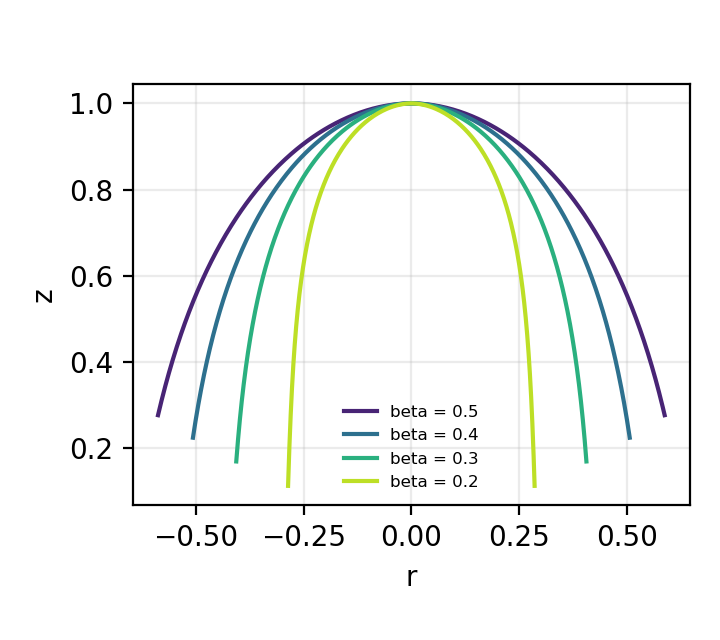
\includegraphics[height=0.38\textheight]{ch10-bell-family}

\scriptsize The bell for $\beta = 0.5, 0.4, 0.3, 0.2$: arc length 1 per half, apex at $z = 1$. Width (tip to tip) $1.17$ at $\beta = 0.5$ and $0.57$ at $0.2$; the bell gets taller as it contracts ($0.72$ to $0.89$), the volume inside it is what is expelled.
\end{column}
\end{columns}
\sourcecredit{The bell of Herschlag and Miller 2011, as the 2013 course taught it; \code{tools/ch10\_figures.py} (formula only).}
\end{frame}

% 24
\begin{frame}{Prescribing contraction and expansion}
\label{fr:jelly2}
\footnotesize ``The value of beta as a function of time during contraction is given by
\[
  \beta(t) = \beta_0 + (\beta_m - \beta_0)\left(\frac{t}{t_0}\right)^{\gamma} .
\]
In the code, gamma is set to 1. The value of beta during expansion is set to
\[
  \beta(t) = \beta_m + (\beta_0 - \beta_m)\left(\frac{t - t_0}{1 - t_0}\right)^{\gamma} .
\]
Similarly, gamma has been set to 1 in the code.'' (2013)
\vspace{1mm}

\footnotesize ``\al{\code{Example\_jellyfish\_curvature}.} The boundary files are generated by \code{generate\_mesh2d.m}. The position of the boundary is calculated for $\beta_0 = 0.5$. Springs are placed between each boundary point to resist stretching. Beams with non-zero curvature are used to prescribe a resting configuration. To generate bell motion, the resting curvature is changed as a function of time in \code{update\_beams.C}. Some work must be done to ensure the beams and springs are sufficiently stiff in order to generate motion.'' (2013)
\vspace{1mm}
\begin{punchbox}
\footnotesize Here $t$ is the time since the pulse began and the period is $1$: the bell contracts for $t_0$ and expands for $1 - t_0$. With $\gamma \neq 1$ the contraction would start slowly and end fast (or the reverse): the shape of the pulse is a second control, which the lab's later studies used. ``Sufficiently stiff'' is slide \ref{fr:stiff}.
\end{punchbox}
\end{frame}

% 25
\begin{frame}[fragile]{The 2013 \code{update\_beams.C} of the jellyfish}
\label{fr:jellycode}
\begin{columns}[T,onlytextwidth]
\begin{column}{0.5\textwidth}
\begin{lstlisting}[style=cpptiny]
//Here I initialize vectors to hold positions to calculate resting curvatures
std::vector<double> Xb_lam(npts_bell);
std::vector<double> Yb_lam(npts_bell);
//These are used to keep track of cycle number and time into the cycle
ptt = floor(current_time/(2*to));   //determine cycle number, starting at 0
pulse_time = current_time-floor(current_time); //determine time since beginning of first pulse

//contract bell
if (pulse_time<to){
	phi = 0;
	beta = betao+(betam-betao)*(pulse_time/to);
	}
//expand bell
else {
	phi = 0;
	beta = betam+(betao-betam)*((pulse_time-to)/(1-to));
	}
\end{lstlisting}
\end{column}
\begin{column}{0.48\textwidth}
\begin{lstlisting}[style=cpptiny]
//Xb and Yb are calculated here and will be used to determine new curvatures
s1=0;
thetaj = -1.55*(1-exp(-(s1)*ds1/beta));
zl = Zs;
ro = 0;
//top of bell
Xb_lam[0]=ro;
Yb_lam[0]=zl;
//right side of bell
for (s1 = 1; s1 <ceil(npts_bell/2); ++s1){
	thetaj = -1.55*(1-exp(-(s1)*ds1/beta));
	zl += ds1*sin(thetaj);
	ro += ds1*cos(thetaj);
	Xb_lam[s1]=ro;
	Yb_lam[s1]=zl;
}
//right side of bell
if (s1<ceil(npts/2)-1){
curv[0]=Xb_lam[s1-1]+Xb_lam[s1+1]-2*Xb_lam[s1];
curv[1]=Yb_lam[s1-1]+Yb_lam[s1+1]-2*Yb_lam[s1];
}
\end{lstlisting}
\end{column}
\end{columns}
\end{frame}

% 25b
\begin{frame}{Reading the 2013 fragments}
\label{fr:jellycode2}
\small Read together: each step, the target shape of the right half is marched out from the apex ($z$ and $r$ accumulate $\Delta s\sin\theta$ and $\Delta s\cos\theta$), and each beam's curvature is the second difference of that shape. What the fragments leave out, IB/10 supplies: the left half (the mirror image), the apex (which in this indexing has no beam across it), \code{npts\_bell}, \code{ds1}, \code{Zs}, \code{to}, \code{betao}, \code{betam} and the stiffnesses. Two inconsistencies: \code{pulse\_time} assumes a period of 1 while \code{ptt} assumes $2t_0$ (equal only for $t_0 = 0.5$, which IB/10 ships); and the slide titled \code{update\_beam.C} is the same file as \code{update\_beams.C}. \code{phi} is set and never used.
\end{frame}

% 26
\begin{frame}[fragile]{IB/10, the jellyfish bell: what it is}
\label{fr:jelly3}
\vspace{-1mm}
\begin{columns}[T,onlytextwidth]
\begin{column}{0.52\textwidth}
\footnotesize One curve of $2n + 1 = 257$ points from the left tip through the apex to the right tip, $\Delta s = 1/128$ (half a cell of the $256$ finest grid in a $4\times4$ box, walls all round), springs between neighbours ($K = 1000$) and a beam at every interior point with the resting bell's second differences in the file ($k_b = 1$). Dimensionless units (chapter 8b): arc length 1 per half, period 1, $\rho = 1$, $\mu = 0.01$. Nothing is tethered.
\begin{lstlisting}[style=cpptiny]
// update_beams.cpp (IB/10): the shape for this step, then its second differences
const double pulse_time = current_time - std::floor(current_time / period) * period;
beta = (pulse_time < t_contract) ? beta_0 + (beta_m - beta_0) * (pulse_time / t_contract)
                                 : beta_m + (beta_0 - beta_m) * ((pulse_time - t_contract) / (period - t_contract));
std::vector<double> r, z;
bell::shape(beta, r, z);                  // bell_geometry.h: the right half, apex to tip
for (int i = 0; i < npts; ++i)            // the whole curve, the left half mirrored
{   const int k = std::abs(i - bell::n);
    X[i] = (i < bell::n ? -r[k] : r[k]);  Y[i] = z[k]; }
...
curv[0] = X[i - 1] - 2.0 * X[i] + X[i + 1];
curv[1] = Y[i - 1] - 2.0 * Y[i] + Y[i + 1];
\end{lstlisting}
\end{column}
\begin{column}{0.46\textwidth}
\scriptsize \code{PERIOD}, \code{T\_CONTRACT} ($0.5$), \code{BETA\_0} ($0.5$) and \code{BETA\_M} ($0.2$) are input keys; the geometry is in \code{bell\_geometry.h}, shared by the generator's logic and the update function, as \code{pump\_geometry.h} was in IB/11.
\vspace{1mm}

\scriptsize \al{Why these numbers.} The first version had the bell at the $512$ grid ($\Delta s = 1/256$, 513 points), $k_b = 10^{-3}$ and $K = 1$: it ran, and did nothing. The bending force per unit length of a beam asked to change its curvature by $\Delta\kappa$ is about $k_b\,\Delta\kappa/L^2$; to move the fluid it must beat $\rho U^2$, which for a bell of size 1 contracting in half a period is of order 1. So $k_b \sim 1$, a thousand times stiffer, and springs stiff enough not to stretch under it ($K \sim 1000$). That stiffness at $\Delta s = 1/256$ would need $\Delta t \sim 10^{-5}$ (next slide); halving the resolution gives $\Delta t = 5\times10^{-5}$ and 40,000 steps for two pulses, about 15 minutes on 2 cores.
\vspace{1mm}

\scriptsize Changes from 2013: one curve instead of an apex with two sides; parameters in the input; the mirror done once per step; structure-relative indices; \code{IBTK::Vector}.
\end{column}
\end{columns}
\end{frame}

% 27
\begin{frame}{IB/10: the bell pulsing and moving}
\label{fr:jelly4}
\begin{columns}[T,onlytextwidth]
\begin{column}{0.64\textwidth}
\centering
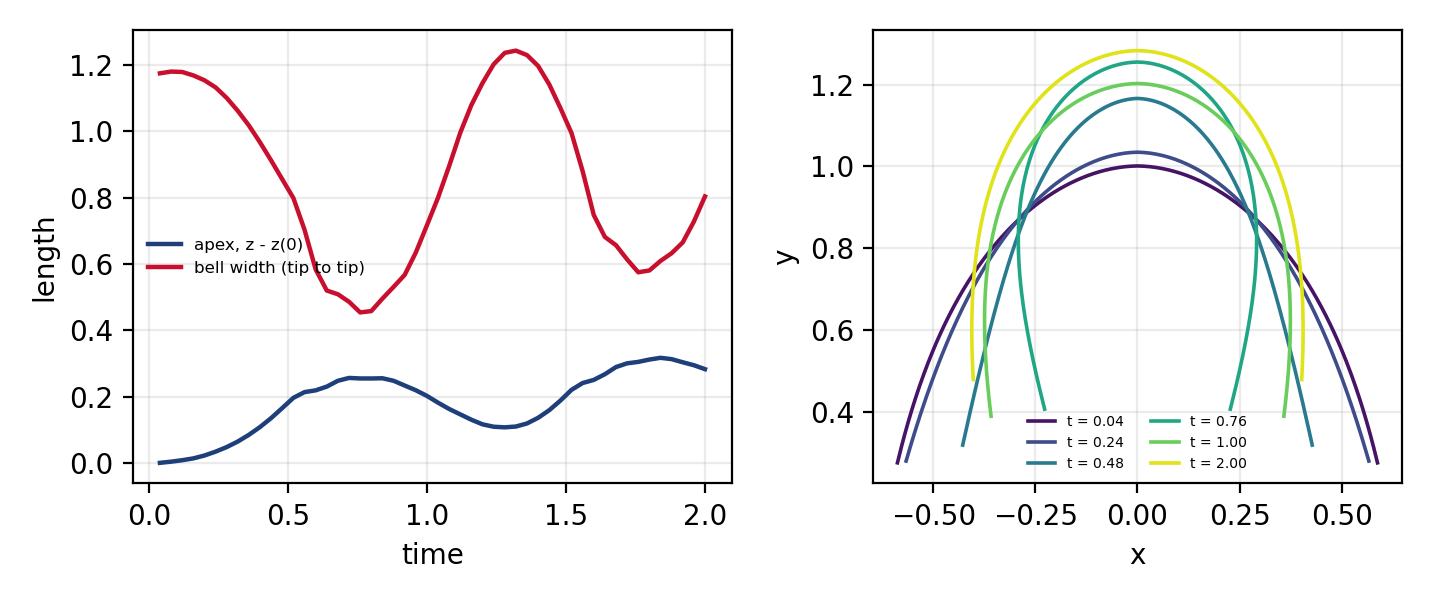
\includegraphics[width=\textwidth]{ch10-jelly-swim}
\end{column}
\begin{column}{0.34\textwidth}
\scriptsize Left: the apex's height above its start and the bell's width against time. Right: the bell at six times.
\vspace{1mm}

\scriptsize Measured: the width falls from $1.17$ to $0.45$ (the shape asks for $0.57$) at $t = 0.75$, a quarter period after the contraction ends at $0.5$, and recovers to $1.24$ at $1.3$; the bell follows its curvature with that lag and overshoots a little. The apex rises $0.25$ during the first contraction, falls back to $0.11$ during the expansion (the recoil of the fluid drawn back into the bell) and ends $0.28$ above its start after two pulses: a net $0.14$ bell-lengths per pulse, upward, with nothing but the changing curvature to drive it.
\vspace{1mm}

\scriptsize Chapter 26 renders the vortex rings each contraction sheds (\code{Omega} in VisIt); chapter 11 reads the forces; chapter 8b's $\mathrm{Re}$ and $\mathrm{St}$ are the knobs the lab's jellyfish papers turned.
\end{column}
\end{columns}
\sourcecredit{IB/10 with IBAMR 0.19.0; \code{tools/ch10\_figures.py}.}
\end{frame}

% 28
\begin{frame}{``Sufficiently stiff'': stiffness against time step}
\label{fr:stiff}
\vspace{-2mm}
\footnotesize The one trade-off every curvature-driven body meets:
\begin{itemize}
  \item \al{Stiff enough to move the fluid.} A beam asked to change curvature by $\Delta\kappa$ pushes with about $k_b\,\Delta\kappa/L^2$ per unit length; it must exceed the fluid's resistance, inertial ($\rho U^2$) or viscous ($\mu U/L$), or the body ignores its own curvature (IB/10's first version; IB/09's 44 mm lag). Chapter 8b: $k'_b = k_b/(\rho U^2 L^3)$ should be of order one or more.
  \item \al{Soft enough for the time step.} The explicit IB scheme (chapter 5) is stable only if $\Delta t$ resolves the stiffest oscillation. For beams the file stiffness $k_b/\Delta s^3$ acts on a point that drags about $\rho\,\Delta x\,\Delta s$ of fluid, so the frequency scales as $\sqrt{k_b/(\rho\,\Delta s^4\,\Delta x)}$ and the number of steps per period as
  \[
    \frac{T}{\Delta t} \;\propto\; \left(\frac{L}{\Delta s}\right)^2 \sqrt{\frac{L}{\Delta x}}\;\sqrt{k'_b}\,,
  \]
  which is why the resolution, not the physics, sets the cost: IB/10 at $L/\Delta s = 128$ needs 20,000 steps per pulse; at 256 it would need 80,000.
  \item \al{Measured points} (this series): IB/03's leaf, $k_b/\Delta s^3 = 5.3\times10^6$ at $\rho = 1000$, runs at $\Delta t = 10^{-4}$; ten times stiffer needs $2.5\times10^{-5}$ (chapter 8a); IB/09 at four times stiffer runs at $5\times10^{-5}$; IB/10 at $k_b/\Delta s^3 = 2.1\times10^6$, $\rho = 1$, $\Delta x = 1/64$ runs at $5\times10^{-5}$.
\end{itemize}
\begin{punchbox}
\scriptsize ``Some work must be done to ensure the beams and springs are sufficiently stiff in order to generate motion'' (2013) means: raise $k_b$ until the body follows its curvature within a fraction of the period, then lower $\Delta t$ until the run is stable, then wait. Chapter 16 is about the aborts you meet on the way.
\end{punchbox}
\end{frame}

% 29
\begin{frame}{Orientation: when the body turns}
\label{fr:orientation}
\small The preferred curvature is a vector in laboratory coordinates (slides \ref{fr:nonzero}, \ref{fr:worksheet}). Three cases:
\begin{itemize}
  \item \al{The body does not rotate} (IB/09's clamp fixes its direction; IB/10's bell is symmetric and swims straight): write $\mathbf{C}_i$ once, in laboratory coordinates, and change only its magnitude or the shape it encodes. This is what the examples do.
  \item \al{The body rotates by a known angle} (a fin flapping about a hinge whose motion you prescribe): rotate the preferred second differences by that angle each step, $\mathbf{C}_i(t) = \mathcal{R}(\alpha(t))\,\mathbf{C}_i^{\mathrm{body}}$. Second differences rotate like vectors, so one $2\times2$ rotation per beam does it.
  \item \al{The body rotates freely} (a swimmer that yaws): measure the body's orientation from its own points each step (the direction from the apex to the midpoint of the tips, say, or a least-squares axis), and rotate $\mathbf{C}_i^{\mathrm{body}}$ by it. Then the preferred shape turns with the body, and the beams never fight a rotation. The 2013 note ``IBAMR has no rotation-aware method'' still holds: the generator writes the laboratory frame, and this bookkeeping is yours.
\end{itemize}
\vspace{1mm}
\begin{punchbox}
\footnotesize The angle form of slide \ref{fr:angle} ($C = R_{pq}R_{qr}\sin\theta_{\mathrm{desired}}$) is invariant by construction; IB2d offers it, IBAMR's standard force generator does not. A chapter 9b force strategy of your own could implement it in IBAMR.
\end{punchbox}
\end{frame}

% 30
\begin{frame}{What can go wrong}
\label{fr:wrong}
\scriptsize
\begin{tabular}{@{}L{0.3\textwidth}L{0.62\textwidth}@{}}
\toprule
The mistake & What happens\\
\midrule
one curvature number on a beam line in 2D & the initializer stops: ``incomplete beam curvature specification''. All $\mathrm{NDIM}$ or none\\
curvature written in $1/\mathrm{m}$ & a preferred second difference thousands of times too large; the beam snaps into a hairpin or the run aborts. $\|\mathbf{C}\| = \kappa\,\Delta s^2$\\
the second difference of the shape taken at a different spacing & the magnitude scales with $\Delta s^2$: IB/09's ramp is the same mistake made on purpose (a flatter arc)\\
the curvature copied instead of referenced in the update function & nothing moves (slide \ref{fr:api})\\
the global \code{lag\_idx} used as the point's number & right for structure 0 only; every other structure gets the wrong angles\\
a beam too soft for the fluid & the body ignores its curvature (IB/10's first version), or lags it (IB/09 with the leaf's stiffness)\\
a beam stiff enough, at the old time step & ``Time step size change encountered'' or NaN within a few hundred steps (chapter 16)\\
the preferred shape in the body frame while the body rotates & the beams fight the rotation; a free swimmer straightens or spins (slide \ref{fr:orientation})\\
a closed loop with the curvature columns left out of the last beam & the join is pushed straight while the rest is curved: a kink at the seam. Chapter 6's closed-loop beam across the join needs its columns too\\
\bottomrule
\end{tabular}
\end{frame}

% 31
\begin{frame}{Homework}
\label{fr:hw}
\begin{columns}[T,onlytextwidth]
\begin{column}{0.56\textwidth}
\footnotesize From the 2013 course and this chapter (Appendix C collects the full set):
\begin{enumerate}
  \item IB/09: make the beam curl into a half circle instead of a quarter (change $\varphi_i$'s range and $R_{\mathrm{final}}$), and into a quarter circle the other way (the sign of $C_2$).
  \item IB/09: give the beam the quarter circle's curvature in the \code{.beam} file from the start (the worksheet's recipe) and no update function. How long does it take to reach its shape, and how does that compare with the ramp?
  \item IB/10: change $t_0$ to $0.3$ (a fast contraction, slow expansion) and compare the distance travelled per pulse; then $\beta_m = 0.3$ (a weaker contraction).
  \item IB/10: double $\mu$ (halve the Reynolds number) and say what happens to the swimming speed; Herschlag and Miller 2011 is the reference.
  \item Write the invariant angle form of the bending energy as a chapter 9b force strategy, and show that a rotated IB/09 beam curls the same way with it.
\end{enumerate}
\end{column}
\begin{column}{0.42\textwidth}
\begin{punchbox}
\scriptsize What to hand in: the \code{.beam} lines or the update function's curvature lines you changed, the generator loop, the step you had to use, and one VisIt frame per run with the shape and the vorticity.
\end{punchbox}
\scriptsize Extension: compute the bending energy $E_b$ of IB/09 from the \code{X.*} files (chapter 11) and plot it against time; it should peak while the curvature is still changing.
\end{column}
\end{columns}
\end{frame}

% 32
\begin{frame}{Rules of thumb}
\label{fr:thumb}
\small
\begin{itemize}
  \item A beam pushes its middle point toward $\mathbf{X}_{i-1} + \mathbf{X}_{i+1} - \mathbf{C}_i$ (over 2) and the neighbours the other way; the file stiffness is $k_b/\Delta s^3$.
  \item $\mathbf{C}_i$ is the second difference of the preferred positions: length units, $\|\mathbf{C}\| = \kappa\,\Delta s^2$, direction the normal of the preferred shape, in laboratory coordinates.
  \item A body bent at rest: write its own second differences into columns 5 and 6. A body that moves: recompute them each step in an update function, through a reference.
  \item Count points from the structure's first index; visit ghost nodes; one beam per node unless you made more.
  \item Stiff enough to move the fluid ($k'_b \gtrsim 1$), then a time step that survives it; the cost grows as $(L/\Delta s)^2$.
  \item If the body turns, turn $\mathbf{C}_i$ with it; the angle form of the energy would not need this, and IBAMR does not have it.
  \item Check with the shape against its target (the figures of this chapter) before believing the flow.
\end{itemize}
\end{frame}

% 33
\begin{frame}{Summary}
\label{fr:summary}
\footnotesize
\begin{enumerate}
  \item IB forces are minus the gradient of an energy of the point positions: stretching (springs), bending (beams), tethering (targets). The discrete bending energy is $\frac12 k_b \sum |\mathbf{X}_{i-1} - 2\mathbf{X}_i + \mathbf{X}_{i+1} - \mathbf{C}_i|^2/\Delta s^3$, and its gradient is IBAMR's five lines.
  \item The preferred curvature $\mathbf{C}_i$ is a vector of length units, the second difference of the shape the beam wants; it fixes the orientation as well as the curvature, which the angle form of the 2013 lecture does not.
  \item It goes into the \code{.beam} file as two (or three) extra columns, or into the program through \code{IBBeamForceSpec::getMeshDependentCurvatures()} each step, exactly as chapter 9a changed targets and springs.
  \item IB/09 curls a clamped beam into a quarter circle and shows the lag that fluid inertia imposes; IB/10 makes a bell swim by cycling one shape parameter $\beta(t)$, and shows that the stiffness has to be chosen for the fluid, and the time step for the stiffness.
  \item The cost of a curvature-driven body is set by its resolution, $(L/\Delta s)^2\sqrt{L/\Delta x}$ steps per period; the physics only adds a $\sqrt{k'_b}$.
\end{enumerate}
\begin{homebox}
\footnotesize Next, chapter 11: output and analysis of forces, where the \code{X.*} and \code{F.*} files that measured every figure of chapters 7--10 are read in MATLAB and Python.
\end{homebox}
\end{frame}

% 34
\begin{frame}{What changed since the older course notes}
\label{fr:changed}
\footnotesize
\begin{itemize}
  \item The nine derivation slides that were pictures (the 2013 \emph{Bending in IBAMR} and its 2018 copy) are retyped, with the worksheet, and tied to the lines of \code{IBStandardForceGen.cpp} that implement them; the sign and the $(\Delta s)^4$ versus $\Delta s^3$ bookkeeping are stated from the source.
  \item The two course examples, whose zips are no longer in the folders, are rebuilt as IB/09 and IB/10 from the slides' fragments, with the fixes named on the slides (global index, $n_{\mathrm{pts}}$ versus $n_{\mathrm{pts}} - 1$, the copy of the curvature, the pulse-timing inconsistency, the missing left half and apex beam, hard-coded parameters, \code{update\_beam.C} versus \code{update\_beams.C}).
  \item The 2013 slide's login for a UNC machine is left out; ``the forcing version of IBAMR'' is every version now.
  \item New: the verified force and file-format rules, the orientation recipe for rotating bodies, the stiffness-versus-time-step estimate with measured points, the parameters that did \emph{not} work, and the measured figures.
  \item Chapter 8a's leaf stiffness sweep is referenced instead of repeated.
\end{itemize}
\end{frame}

% 35
\begin{frame}{Recordings (listed, not incorporated)}
\label{fr:videos}
\small The front matter's video list (chapter 0.1) has no recording of the 2013 bending or jellyfish lectures. The 2018 recordings of chapter 9a's material (\code{5-Video-SpringsTargetsPart1.mp4}, \code{Part2.mp4}, 2018-02-14) cover the update-function pattern that \code{update\_beams} follows. The lab's \emph{TubeHeart} videos (2015, listed in the front matter under the IBFE projects) show a bell-less heart tube; the jellyfish animations of the 2011 paper are on the journal's site.
\end{frame}

% 36
\begin{frame}{References}
\label{fr:refs}
\scriptsize
\begin{itemize}
  \item IBAMR 0.19.0: \code{src/IB/IBStandardForceGen.cpp} (the beam force), \code{src/IB/IBStandardInitializer.cpp} (\code{readBeamFiles}, the curvature columns and \code{uniform\_beam\_curvature}), \code{include/ibamr/IBBeamForceSpec.h}. \url{https://github.com/IBAMR/IBAMR}
  \item The examples of this series: IB/09 curling beam (\code{update\_beams.cpp}, \code{generate\_mesh2d.py}/\code{.m}, README with the measured lag), IB/10 jellyfish bell (\code{bell\_geometry.h}, \code{update\_beams.cpp}, generators, README with the parameters that did and did not work), IB/03 and chapter 8a's sweep; \code{tools/ch10\_figures.py}.
  \item C. S. Peskin, \emph{The immersed boundary method}, Acta Numerica 11 (2002) 479--517 (the energy formulation of the forces).
  \item G. Herschlag and L. A. Miller, \emph{Reynolds number limits for jet propulsion: a numerical study of simplified jellyfish}, J.\ Theor.\ Biol.\ 285 (2011) 84--95 (the bell shape and the pulse of IB/10).
  \item Sources: \emph{Bending in IBAMR} (MATH 769, February 19, 2013, 20 slides) with \code{Discrete\_curvature.xlsx}; \emph{Specific example of jellyfish swimming by prescribing curvature} (MATH 769, February 26, 2013, 8 slides); \emph{IBAMR Tutorial: Changing Curvature} (public folder 6, edition of 2018, 28 slides).
\end{itemize}
\end{frame}

\end{document}
